\documentclass[12pt]{article}
\usepackage[spanish]{babel}
\usepackage{apacite}
\usepackage[utf8]{inputenc}
\usepackage{amsmath}
\usepackage{mathrsfs}
\usepackage{listings}
\usepackage[usenames]{color}
\definecolor{gray97}{gray}{.97}
\definecolor{gray75}{gray}{.75}
\definecolor{gray45}{gray}{.45}
\definecolor{azul1}{RGB}{141,198,163}
\definecolor{azul2}{RGB}{24,107,122}
\definecolor{verde1}{RGB}{44,186,34}
\usepackage{textcomp}
\lstset{
		frame=Ltb,
		framerule=1pt,
		framextopmargin=3pt,
		framexbottommargin=3pt,
		framexleftmargin=0.4cm,
		framesep=0pt,
		rulesep=.4pt,
		backgroundcolor=\color{gray97},
		rulesepcolor=,
        tabsize=4,
        rulecolor=\color{azul1},
        basicstyle=\scriptsize\rmfamily,
        upquote=true,
        aboveskip={1.5\baselineskip},
        columns=fixed,
        showstringspaces=false,
        extendedchars=true,
        breaklines=true,
        prebreak = \raisebox{0ex}[0ex][0ex]{\ensuremath{\hookleftarrow}},
        showtabs=false,
        showspaces=false,
        showstringspaces=false,
        identifierstyle=\rmfamily,
        keywordstyle=\color[rgb]{0,0,1},
        commentstyle=\color[rgb]{0.133,0.545,0.133},
        stringstyle=\color[rgb]{0.627,0.126,0.941},
        keywordstyle=\bfseries,
        %
		numbers=left,
		numbersep=15pt,
		numberstyle=\tiny,
		numberfirstline = false,
		breaklines=true,
		}
\usepackage{graphicx}
\usepackage[colorinlistoftodos]{todonotes}
\usepackage{natbib} %citas bibliograficas estilo APA :p
\usepackage{eso-pic}
\usepackage{avant}
\usepackage[top=2cm,bottom=2cm,left=2.5cm,right=3cm,headsep=8pt,a4paper]{geometry}
\usepackage{fancyhdr}
\pagestyle{fancy}
\fancyhf{}
%\fancyhead[LE,RO]{}
\fancyhead[RE,LO]{Control Digital y Aplicaciones}
\fancyfoot[CE,CO]{\leftmark}
\fancyfoot[LE,RO]{\thepage}
\renewcommand{\headrulewidth}{2pt}
\renewcommand{\footrulewidth}{1pt}
\usepackage{tabu}
\usepackage{array}
\usepackage{multirow}
\usepackage{amssymb}
\usepackage{makeidx}
\graphicspath{ {images/} }
\usepackage{wrapfig}
\usepackage{enumerate}
\usepackage{amsmath,tikz}
\usetikzlibrary{matrix}
\usepackage{steinmetz}
\newcommand*{\horzbar}{\rule[0.05ex]{2.5ex}{0.5pt}}
\usepackage{calc}
\date{\today}


\begin{document}

\begin{titlepage}
\newcommand{\HRule}{\rule{\linewidth}{0.5mm}} 
\center
\textsc{\LARGE  Benemérita Universidad \\[0.2cm] Autónoma de Puebla}\\[1.5cm] 

\includegraphics[width=4cm]{IMAGENES/escudo}\\[1cm]
\textsc{\Large Facultad de Ciencias de la Electrónica}\\[0.5cm] 
\textsc{\large Licenciatura en Electrónica}\\[0.5cm]
\HRule \\[0.4cm]
{ \huge \bfseries Tarea 1}\\[0.4cm] 
\HRule \\[1.5cm]
\begin{minipage}{\textwidth}
\center 

\emph{Profesor:} \\
Gutierres Arias Jose Eligio Moises, \\[1cm]
\vspace{10mm}
\begin{tabular}{ll}
\emph{Alumno:} & \emph{Número de Matrícula:}\\
Hanan Ronaldo Quispe Condori  & 555010653 \\
\end{tabular}
\end{minipage}\\[2cm]
%\today
\end{titlepage}

%\newpage
%~\vfill
%\thispagestyle{empty}
%\begin{figure}[hbtp]


%\includegraphics[width=4cm]{IMAGENES/motordc}
%\end{figure}
%\noindent \textsc{Trabajo Encargado: Problemas en MatLab \\ Máquinas Eléctricas \\ Universidad Nacional de San Antonio abad del Cusco}\\
%noindent \textsc{Ingeniería Electrónica }\\
%\noindent \textit{Tercera revisión, \today}

%\tableofcontents indice bloqueado xD

\newpage
\section{Transformada Z}
\subsection{Transformada Z Bilateral}
La transformada Z surge de la transformada de Fourier discreta, esta se define de la siguiente manera.
\begin{equation}
    \begin{split}
        %A&=J_{B}L(J_{p}+J_{1})\\
        \displaystyle\sum_{n=-\infty}^\infty\,x[n]e^{-j\omega n}\\
    \end{split}
    \label{eq:dft}
\end{equation}
Se tendrá la definición de la transformada Z tomando variable $z=re^{j\omega}$, bajo esta consideranción, la ecuación \ref{eq:dft} quedara de la siguiente forma, tomemos en cuenta que cuando $r=1$ la transformada Z será la transformada de Fourier discreta (\cite{schafer1989discrete}).
\begin{equation}
    \begin{split}
        \displaystyle\sum_{n=-\infty}^\infty\,x[n]z^{-n}\\
    \end{split}
    \label{eq:zt}
\end{equation}
Tomaremos una nueva notación para ecuación \ref{eq:zt} 
\begin{equation}
    \begin{split}
        \mathscr{Z}\{x[n]\}&=\displaystyle\sum_{n=-\infty}^\infty\,x[n]z^{-n}=X(z)\\
    \end{split}
    \label{eq:zt1}
\end{equation}
La sumatoria \ref{eq:zt} convergerá solo si se cumple que
\begin{equation}
    \begin{split}
        \displaystyle\sum_{n=-\infty}^\infty\,|x[n]||z^{-n}|<\infty\\
        \displaystyle\sum_{n=-\infty}^\infty\,|x[n]||(re)^{-j\omega n}|<\infty\\
        \displaystyle\sum_{n=-\infty}^\infty\,|x[n]r^{-n}|<\infty\\
    \end{split}
    \label{eq:zt2}
\end{equation}
Para que la ecuación \ref{eq:zt2} se cumpla la secuencia debe ser absolutamente sumable, debemos encontrar el rango de valores de $r$ para que esto se cumpla, con este objeto, procederemos a operar en \ref{eq:zt2} como sigue.
\begin{equation}
    \begin{split}
        X(z)&\leq\displaystyle\sum_{n=-\infty}^{-1}\,|x(n)r^{-n}|+\displaystyle\sum_{n=0}^\infty\,|x(n)r^{-n}|\\
        X(z)&\leq\displaystyle\sum_{n=}^\infty\,|x(-n)r^{n}|+\displaystyle\sum_{n=0}^\infty\,|x(n)r^{-n}|\\
    \end{split}
    \label{eq:zt3}
\end{equation}
De \ref{eq:zt3} podemos sacar las siguientes relaciones para $n$, $1\leq n<\infty$ y $0\leq n<\infty$, estas relaciones nos daran una region donde la transformada Z convergerá, si analizamos esta region, se podra obtener información sobre la secuencia
\begin{itemize}
    \item Secuencia de longitud finita $0<|z|<\infty$
    \item Secuencia limitada por la derecha $R_{x-}<|z|<\infty$
    \item Secuencia limitada por la izquierda $0<|z|<R_{x+}$
    \item Secuencia bilateral $R_{x-}<|z|<R_{x+}$     
\end{itemize}
\subsubsection{Propiedades de la Transformada Z}
\textbf{Linealidad}
\vspace{5mm}

%\setlength{\parindent}{10ex}
Esta propiedad establece que\par

\begin{equation}
    \begin{split}
        \displaystyle\sum_{n=-\infty}^{\infty}\,(ax_{1}[n]+bx_{2}[n])z^{-n}&=a\displaystyle\sum_{n=-\infty}^{\infty}\,x_{1}[n]z^{-n}+b\displaystyle\sum_{n=-\infty}^{\infty}\,x_{2}[n]z^{-n}\\
    \end{split}
    \label{eq:lineal}
\end{equation}

\textbf{Desplazamiento en el Tiempo}
\vspace{5mm}

%\setlength{\parindent}{10ex}
Esta propiedad establece que\par

\begin{equation}
    \begin{split}
        x[n-n_{0}]\xrightarrow{\mathscr{Z}}z^{-n_{0}}X(z)\\
    \end{split}
    \label{eq:despla_time}
\end{equation}

Demostración
\begin{equation}
    \begin{split}
        X(Z)&=\displaystyle\sum_{n=-\infty}^{\infty}\,x[n-n_{0}]z^{-n}\\
    \end{split}
    \label{eq:despla_time1}
\end{equation}
Haciendo cambio de variable $m=n-n_{0}$ en \ref{eq:despla_time1} se tendrá
\begin{equation}
    \begin{split}
        Y(Z)&=\displaystyle\sum_{n=-\infty}^{\infty}\,x[m]z^{m+n_{0}}\\
        Y(Z)&=z^{-m_{0}}X(Z)\\
    \end{split}
    \label{eq:despla_time2}
\end{equation}

\textbf{Propiedad de Convolución}
\vspace{5mm}

%\setlength{\parindent}{10ex}
La convolución de dos secuencias, equivale a la multiplicación de sus respectivas transformadas Z.\par
\begin{equation}
    \begin{split}
        x_{1}[n]*x_{2}[n]\xrightarrow{\mathscr{Z}}X_{1}(Z)X_{2}(Z)\\
    \end{split}
    \label{eq:convolu}
\end{equation}
Demostración

Sea la convolución de $x_{1}[n],x_{2}[n]$ en tiempo discreto
\begin{equation}
    \begin{split}
        y[n]=\displaystyle\sum_{k=-\infty}^{\infty}\,x_{1}[k]x_{2}[n-k]\\
    \end{split}
    \label{eq:convolu_demo}
\end{equation}
Calculando la transformada Z de la ecuación \ref{eq:convolu_demo} se tendrá.
\begin{equation}
    \begin{split}
        Y(Z)=\displaystyle\sum_{n=-\infty}^{\infty}\,(\displaystyle\sum_{k=-\infty}^{\infty}\,x_{1}[k]x_{2}[n-k])z^{-n}\\
    \end{split}
    \label{eq:convolu_demo1}
\end{equation}
Haciendo cambio de variable $m=n-k$ e intercambiando el orden de la suma se tendrá
\begin{equation}
    \begin{split}
        Y(Z)&=\displaystyle\sum_{k=-\infty}^{\infty}\,x_{1}[k](\displaystyle\sum_{m=-\infty}^{\infty}\,x_{2}[m]z^{-m})z^{-k}\\
        Y(Z)&=(\displaystyle\sum_{k=-\infty}^{\infty}\,x_{1}[k]z^{-k})X_{2}(Z)\\
        Y(Z)&=X_{1}(Z)X_{2}(Z)\\
    \end{split}
    \label{eq:convolu_demo2}
\end{equation}

\textbf{Diferenciación}
\vspace{5mm}

%\setlength{\parindent}{10ex}
Esta propiedad estipula que\par
\begin{equation}
    \begin{split}
        nx_{1}[n]\xrightarrow{\mathscr{Z}}-z\frac{dX(z)}{dz}\\
    \end{split}
    \label{eq:dif}
\end{equation}
Demostración
Sea la transformada Z de la secuencia $x[n]$ 
\begin{equation}
    \begin{split}
        Y(Z)=\displaystyle\sum_{n=-\infty}^{\infty}\,x[n]z^{-n}\\
    \end{split}
    \label{eq:dif_demo}
\end{equation}
Derivando la ecuación \ref{eq:dif_demo} con respecto a $z$ y multiplicando por $-z$
\begin{equation}
    \begin{split}
        -z\frac{dX(z)}{dz}&=-z\displaystyle\sum_{n=-\infty}^{\infty}\,(-n)x[n]z^{-n-1}\\
        -z\frac{dX(z)}{dz}&=\displaystyle\sum_{n=-\infty}^{\infty}\,nx[n]z^{-n}\\
    \end{split}
    \label{eq:dif_demo1}
\end{equation}
\subsection{Transformada Z Unilateral}
La transformada bilateral necesita ser definida para el rango completo de $-\infty<n<\infty$, este requerimiento impide que sea usada para la resolución de problemas, los sistemas descritos por ecuaciones de diferencias con condiciones iniciales diferentes a cero, esto ya que la entrada aplicada en un tiempo finito $n_{0}$ esta especificada para $n\ge n_{0}$, pero no necesariamente será cero para $n\le n_{0}$, por lo que la transformada bilateral no puede ser usada; para solucionar este problema, se tendrá que definir la transformada Z unilateral. \cite{proakis1996digital}
\begin{equation}
    \begin{split}
        X^+(z)&=\displaystyle\sum_{n=0}^{\infty}\,x[n]z^{-n}\\
    \end{split}
    \label{eq:zt_unilateral}
\end{equation}
La notación antes usada para la transformada Z cambiara a $\mathscr{Z}^+\{x[n]\}$, esta transformada difiere de la transformada bilateral en el limite inferior de la sumatoria, el cual es siempre cero.

Casi todas las propiedades estudidadas para la transformada bilateral se cumplen tambien para la transformada unilateral, a excepción de la propiedad de desplazamiento en el tiempo.

\textbf{Retardo en el Tiempo}
\vspace{5mm}

Sea 
\begin{equation}
    \begin{split}
        x[n]\xrightarrow{\mathscr{Z}^+}X^+(z)\\
    \end{split}
    \label{eq:uzt_delay}
\end{equation}

Sabemos que $x[n]$ sera causal entonces se tendrá

\begin{equation}
    \begin{split}
        \mathscr{Z}^+\{x[n-k]\}&=z^{-k}[\displaystyle\sum_{l=-k}^{-1}\,x[l]z^{-l}+\displaystyle\sum_{l=0}^{\infty}\,x[l]z^{-l}]\\
        \mathscr{Z}^+\{x[n-k]\}&=z^{-k}[\displaystyle\sum_{l=-1}^{-k}\,x[l]z^{-l}+X^+(z)]\\
    \end{split}
    \label{eq:uzt_delay1}
\end{equation}
Haciendo el cambio de variable $n=-l$ se tendrá
\begin{equation}
    \begin{split}
        \mathscr{Z}^+\{x[n-k]\}&=z^{-k}[\displaystyle\sum_{n=1}^{k}\,x[-n]z^{n}+X^+(z)], \quad k>0\\
    \end{split}
    \label{eq:uzt_delay2}
\end{equation}

\textbf{Adelanto en el Tiempo}
\vspace{5mm}

Sea 
\begin{equation}
    \begin{split}
        x[n]\xrightarrow{\mathscr{Z}^+}X^+(z)\\
    \end{split}
    \label{eq:uzt_advance}
\end{equation}

Sabemos que $x[n]$ sera causal entonces se tendrá

\begin{equation}
    \begin{split}
        \mathscr{Z}^+\{x[n+k]\}&=z^{-k}\displaystyle\sum_{n=0}^{\infty}\,x[n+k]z^{-n}=z^{k}\displaystyle\sum_{l=k}^{\infty}\,x[l]z^{-l}\\
    \end{split}
    \label{eq:uzt_advance1}
\end{equation}
Haciendo el cambio de variable $n=k-l$ se tendrá
\begin{equation}
    \begin{split}
        X^+(z)&=\displaystyle\sum_{l=0}^{k-1}\,x[l]z^{-l}+\displaystyle\sum_{l=k}^{\infty}\,x[l]z^{-l}\\
    \end{split}
    \label{eq:uzt_advance2}
\end{equation}
Combinando la ecuación \ref{eq:uzt_advance2} obtendremos finalmente
\begin{equation}
    \begin{split}
        \mathscr{Z}^+\{x[n+k]\}&=z^{k}[X^+(z)-\displaystyle\sum_{n=0}^{k-1}\,x[n]z^{-n}], \quad k>0\\
    \end{split}
    \label{eq:uzt_advance3}
\end{equation}
\subsubsection{Transformada Z de Funciones Elementales}

\textbf{Escalon Unitario}
\vspace{5mm}

Sea $x[n]=\mu(n)$

\vspace{5mm}
Usando la definición de la transformada Z unilateral y operando se tendrá.

\begin{equation}
    \begin{split}
        X^+(z)&=\displaystyle\sum_{n=0}^{\infty}\,\mu(n)z^{-n}\\
        X^+(z)&=\displaystyle\sum_{n=0}^{\infty}\,z^{-n}\\
    \end{split}
    \label{eq:ejer1}
\end{equation}

Sabemos que la sumatoria \ref{eq:ejer1} es una serie geométrica cuya fórmula general es
\begin{equation}
    \begin{split}
        \displaystyle\sum_{n=0}^{\infty}\,a_{n}r^{n}&=\frac{a}{1-r}\\
    \end{split}
    \label{eq:ejer11}
\end{equation}

De \ref{eq:ejer11} se tendrá finalmente que 
\begin{equation}
    \begin{split}
        X^+(z)&=\displaystyle\sum_{n=0}^{\infty}\,z^{-n}=\frac{1}{1-z^{-1}}\\
    \end{split}
    \label{eq:ejer12}
\end{equation}

\textbf{Rampa Unitaria}
\vspace{5mm}

Sea $x[n]=n$
Usando la definición de la transformada Z unilateral y operando se tendrá.

\begin{equation}
    \begin{split}
        X^+(z)&=\displaystyle\sum_{n=0}^{\infty}\,nz^{-n}\\
    \end{split}
    \label{eq:ejer2}
\end{equation}

%$$\mathscr{L}\{f(t)\}=F(s)$$
%$$\mathscr{Z}\{f(t)\}=F(s)$$
%\begin{figure}[h]
%    \centering
%        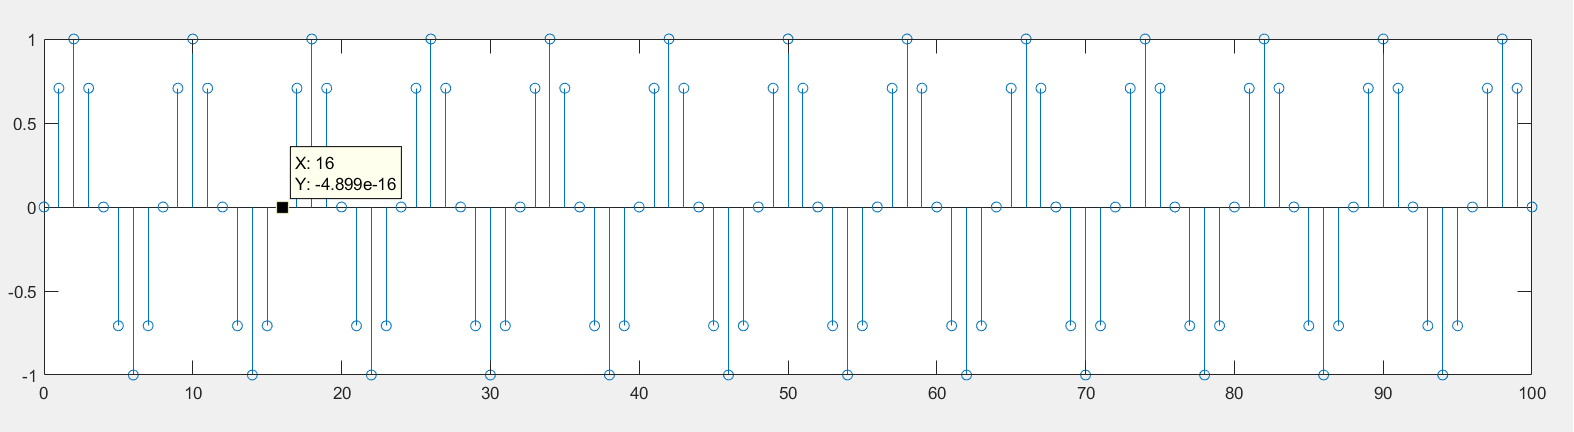
\includegraphics[width=15cm]{IMAGENES/T1_val1.png}
%        \caption{Valor de la muestra 16 para y1.}
%\end{figure}
\bibliographystyle{apacite}
\bibliography{biblio}
\end{document}